\chapter{Introduction}

Since mankind first began making plans, they were based on the available description of the environment. This approach continued into modern times, although the nature of the predictions has changed. People no longer plan which animal to hunt or when to produce stone tools, but instead how many people the postal service should hire for the Christmas season. These decisions require data, and in order to make the right decisions, the data must be available in the right time, in the right context, for the right people and naturally be correct. This makes data one of the most important assets in a company \cite{economist2017_dataoil}. Data allow companies to gain an edge over competitors, analyse clients’ wishes, or improve internal processes. This is where the relevance of this project emerges. 

Swiss Post requires \gls{DA} and \gls{DQ} in its reporting for decision making. This project analyses the current state of a specific data area of Swiss Post and provides steps toward improvements.
This chapter familiarises the reader with the topic. It presents the background of the project at Swiss Post and delves into the motivation behind it. It then further explains the business relevance, demonstrating why it is both important and beneficial for Swiss Post to invest in the topic. Next, the problem statement is addressed, explaining what this project aims to solve. After the problem statement, the scope and limitations of the project are outlined more clearly. Finally, a brief overview of the expected outcomes of the project is provided. This chapter concludes with a preview of the document’s structure.


\section{Background}
\label{IntroBackground}
Swiss Post is Switzerland’s national service provider, active not only in mail and parcel logistics but also in passenger transport (PostAuto), financial services (PostFinance), and various digital and e-government solutions. Its workforce of approximately 45’000 employees and nationwide infrastructure move millions of items and people every day, supported by highly automated sorting centres and extensive data flows \cite{postGeschäftsbericht2024}. In such a diversified organisation, \gls{analyticalreporting} is essential for strategic steering, operational planning, and maintaining service quality across business units. The organisational structure of Swiss Post is shown in the following diagram.

\begin{figure}[H]
    \centering
    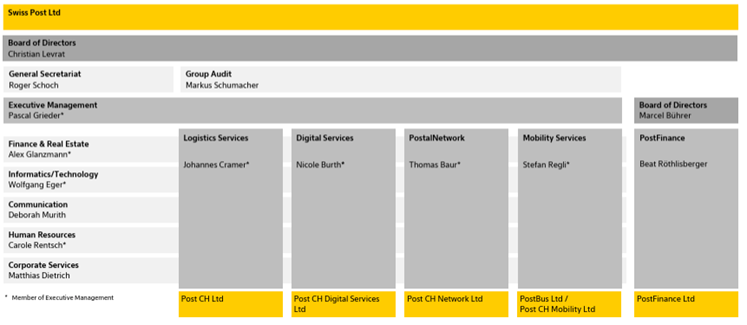
\includegraphics[width=0.8\textwidth]{./content/img/Post_external/OrgStruktur_Online.png}
    \caption{Organisational structure of Swiss Post (online version)}
    \label{fig:orgstruktur_online}
\end{figure}


\subsection*{The full mail piece lifecycle}
Within this large organisation, the project takes place within a specialised team supporting the entire lifecycle of logistics for mail and parcel delivery. In German, this lifecycle covers every step from A to Z, \gls{ASTVZ}, which stands for:
\begin{itemize}
    \item \textbf{A}nnahme: Receiving, where parcels and mail are accepted and registered by Swiss Post to be sent through its network
    \item \textbf{S}ortierung: Sorting, the process during which received mail pieces are separated by destination and routed to the next process step, either further sorting or delivery
    \item \textbf{T}ransport: Transport includes the movement between sorting plants and delivery sectors
    \item \textbf{V}erzollung: Customs clearance handles international parcels and letters, including the required customs checks and documentation
    \item \textbf{Z}ustellung: Delivery is the final process step for every item; it is delivered by the staff of Swiss Post
\end{itemize}

However, this process is more easily visualised using the future vision of Swiss Post. In particular, the version tailored for the IT domain is well suited to describing the project environment. Starting from the top left with the A or V step, followed by S, T, and Z, the process progresses towards the bottom right.

\begin{figure}[H]
    \centering
    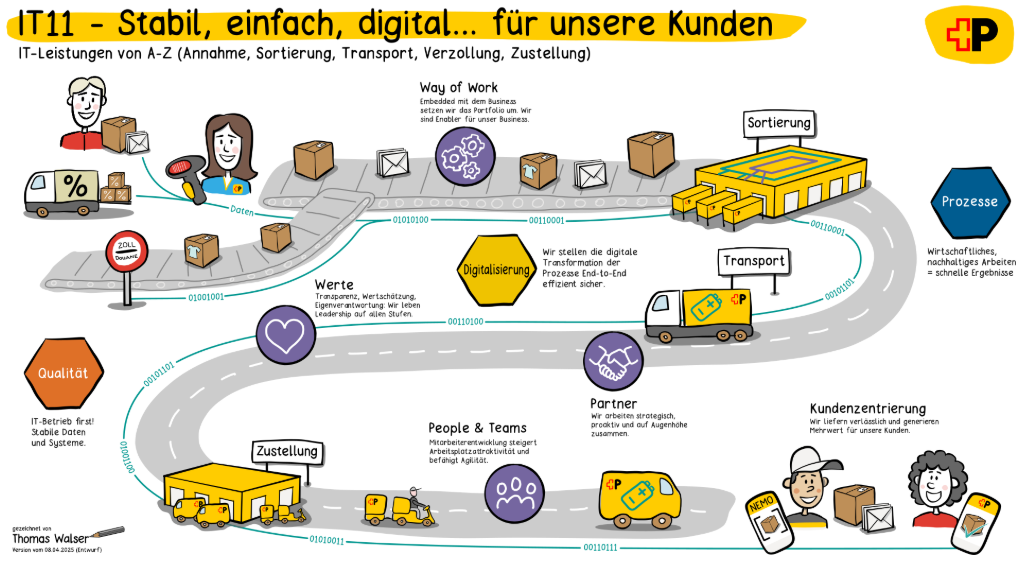
\includegraphics[width=0.8\textwidth]{./content/img/Post_internal/06-12-2025_20-16-16.png}
    \caption{Future way of work illustrating the full postal delivery workflow from receiving an item to delivery.}
    \label{fig:future_way_of_work}
\end{figure}


\subsection*{DWH LS OPS}
\label{IntroDWHLSOPSTasks}

The project team supports the \textbf{D}ata \textbf{W}are\textbf{h}ouse of \textbf{L}ogistic \textbf{S}ervices \textbf{Op}eration\textbf{s} (\gls{DWHLSOPS}). This \textbf{Busi}ness \textbf{Dev}elopment \textbf{Op}eration\textbf{s} (\gls{BizDevOps}) team is located within the organisational structure of the Logistics Services vertical and the Informatics/Technology horizontal. It represents the single source of truth for \gls{analyticalreporting} at Swiss Post. In contrast to operational reporting, which focuses on real-time guidance for operational processes, analytical reporting focuses on aggregated insights for evaluation and planning. Examples of analytical reporting include working time, process time, and aggregations of sorted items. The stakeholders of the team distribute these reports to various task groups within postal services, such as sorting and delivery.

There are two reasons why a deeper understanding of analytical reporting is currently very important. First, the infrastructure for analytical reporting is transitioning from on-premise systems to the cloud. Second, in addition to the migration of reporting, the infrastructure at all Swiss Post \gls{sortingcenter} locations for parcels is undergoing fundamental changes. These changes may include complete modifications of data pipelines, which can make comparisons with previous figures impossible. Therefore, at this critical point in time, it is of utmost importance to maintain users’ trust in the data during this change process. The following figure illustrates the shift from the on-premise setup on the right-hand side to the target architecture using cloud hardware on the left-hand side.

\begin{figure}[H]
    \centering
    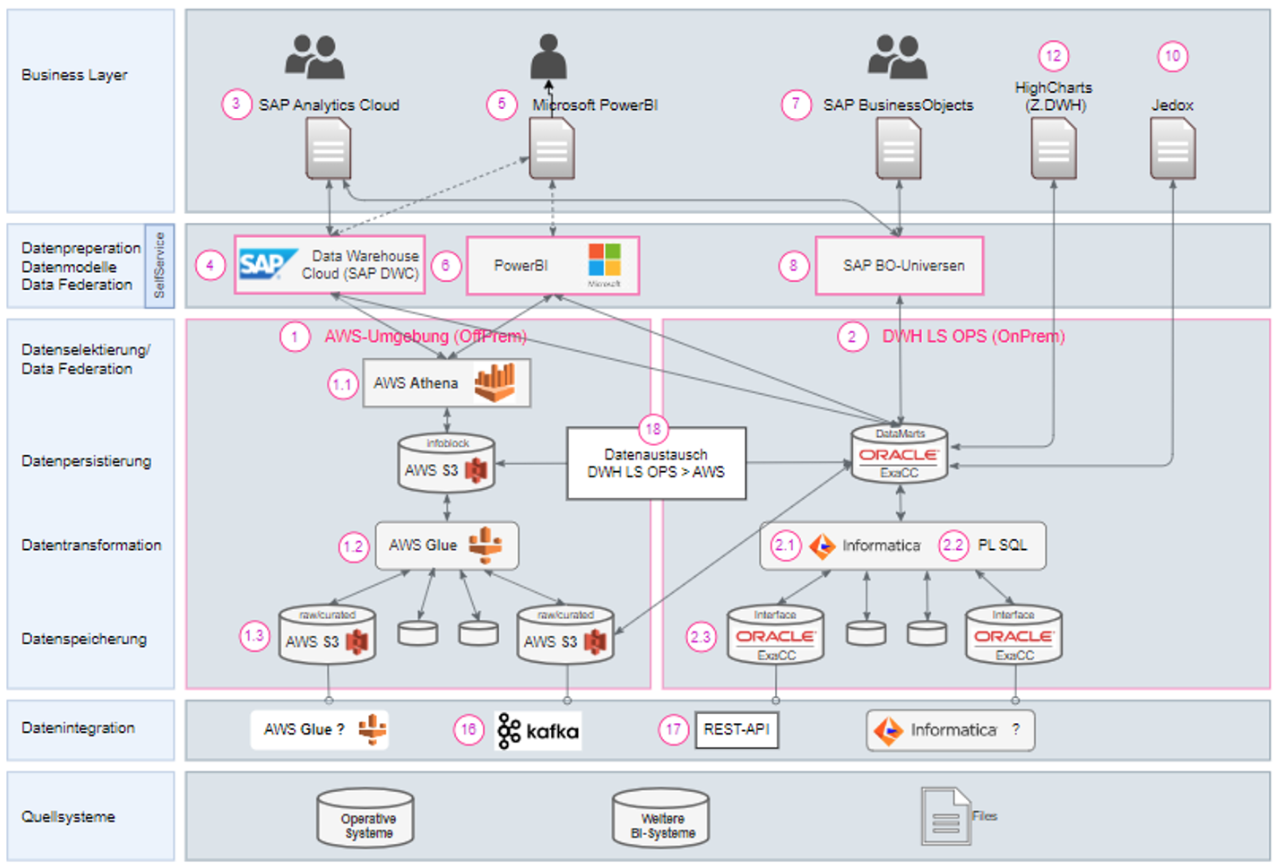
\includegraphics[width=0.8\textwidth]{./content/img/OnPrem_Cloud_Migration.png}
    \caption{The transition from an on-premise setup to a cloud-based target architecture.}
    \label{fig:on_prem_cloud_migration}
\end{figure}


\subsection*{Swiss Post sorting centers are cyber machines}
Swiss Post has built and operate a number of massive sorting centers located across Switzerland. These are far more than just mechanical warehouses or factories. Rather, these sorting centers are massive “cyber facilities” that include high-tech hardware but also high-tech IT systems to keep them running.

While the team handles use cases across the entire postal delivery workflow, this project initially focuses on supporting sorting data flows. Sorting at Swiss Post is the process of consolidating received items in centralised plants, to which letters and parcels are sent from regions across Switzerland. One such plant is located in Härkingen:

\begin{figure}[H]
    \centering
    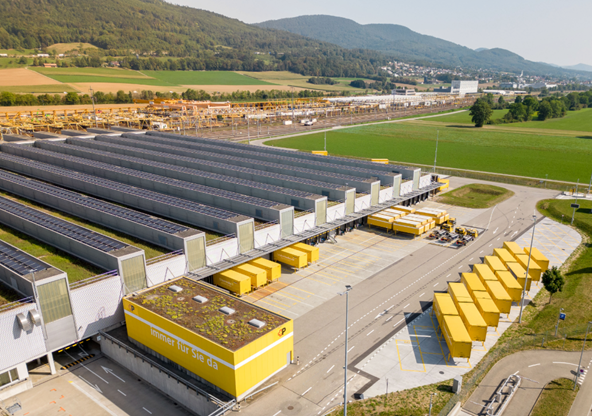
\includegraphics[width=0.8\textwidth]{./content/img/Post_external/Sortierzentrum_Aussen_Vogel.png}
    \caption{Aerial view of the Swiss Post sorting center in Härkingen.}
    \label{fig:sortierzentrum_haerkingen_aerial}
\end{figure}

Mail pieces are handled by workers and placed onto the automated sorting hardware of Swiss Post. This hardware enables the handling of up to 10’000 parcels per hour \cite{SwissPostHarkingenSort}. The system scans the received items and transports them through the plant via conveyor belts to their correct destinations, where they are discharged through chutes. These chutes are shown in the second image, including staff placing the parcels into roll boxes for further processing.

\begin{figure}[H]
    \centering
    \includegraphics[width=0.8\textwidth]{./content/img/Post_ExperienceHub/_DSC4975.jpg}
    \caption{Interior view of the automated sorting system in a Swiss Post sorting center.}
    \label{fig:sortierzentrum_innen_anlage}
\end{figure}
\begin{figure}[H]
    \centering
    \includegraphics[width=0.8\textwidth]{./content/img/Post_ExperienceHub/_DSC4916.jpg}
    \caption{Discharge chutes inside a Swiss Post sorting center, where parcels are released to their designated zones. Then put into rollboxes to get them to next processing steps.}
    \label{fig:sortierzentrum_innen_rutschen}
\end{figure}



\section{Motivation}
\label{IntroMotivation}
\textbf{Data quality} and \textbf{data availability} are central to the successful operations of any company. Even a company working in low-tech or non-IT industries \cite{basedconlDA} has basic but essential data needs, for example, information on who is working where and the addresses of clients and staff. Not having this data in the right quality or available to the right people at the right time will cause problems whenever the data needs to be used.

In the context of ongoing changes to the Swiss Post reporting infrastructure, keeping track of \gls{DA} and \gls{DQ} is challenging. These infrastructure-related changes comprise the construction of new reports, \gls{onetoonemigrations}, and the re-engineering of existing reports.
Since the topic of data quality in the Swiss Post operations area could be built from scratch, as if starting on a \gls{greenfield}, it became an ideal subject for a master’s thesis. 

Furthermore, the topic was not of the highest priority for Swiss Post, but it was still considered a valuable idea to pursue. The medium-priority nature of this project also allowed the topic to be divided into multiple steps, such as working from a PoC to an \gls{MVP} setup. Additionally, the medium priority regarding feature development in this area allowed for well-grounded research on the topic. All these aspects combined made it a suitable project leading to a master’s thesis.
Furthermore, due to the lack of automated data accuracy and data quality checks in the DWH LS OPS environment at the time of defining this project, this topic is highly relevant to the team responsible for both the operational and analytical reports that help guide the company. If the data is incorrect, wrong decisions are made; and if the data is unavailable, management cannot properly lead the staff. Thus, the topic is of high importance and business critical: data quality and availability help Swiss Post continue to deliver reliable services on a daily basis and enable IT to provide better assistance to staff throughout the postal process.

\begin{figure}[H]
    \centering
    
\includegraphics[width=0.8\textwidth]{./content/img/Post_ExperienceHub/Markenshooting_2021_Tessin_LS_059.png}
    \caption{Main customer touch point, delivery of a parcel}
    \label{fig:intro_parcel_mailman}
\end{figure}

\section{Problem statement}
The two key problems addressed in this project are, first, that data quality in this area of Swiss Post has so far been handled in an ad hoc manner, without formal definitions, frameworks, or an agreed set of KPIs; and second, that data quality is handled manually by the business at a \gls{highlevel} rather than being automated by the IT department. Both of these problems lead to issues not being detected early and to longer reaction times. As a further consequence, delays in data processing are not identified and targeted for systematic resolution, which in turn reduces management confidence in the reports. All of this prevents continuous improvement, as the current checks are neither documented nor stored in a way that allows follow-up analysis or structured refinement.


\section{Scope and boundaries}
This research focuses on the data availability and data quality challenges of the \gls{DWHLSOPS} \gls{BizDevOps} \gls{ASTV} teams at Swiss Post described in section \ref{IntroBackground}. To simplify the scope of this work, the first step of data retrieval, such as how data is stored from \gls{KafkaTopics}, is excluded. The scope begins with the curated and reporting layers in the \gls{ETL} process of the retrieved data. The aim of this project is to specifically provide solutions for the mentioned teams and not to offer a general solution or framework for the entire Swiss Post.


\section{Expected outcome}
The high-level goal of this master’s thesis pre-project is to demonstrate that automated data quality checks provide additional safety and can be calibrated to the needs of the business. Automated data quality checks refer to checks executed daily or upon data load, which are always carried out by systems without the need for manual interaction. More specifically, the project focuses on establishing the foundations for this goal by analysing the current situation and developing a proof of concept (\gls{PoC}). It will carefully document and explain the steps taken toward the proof of concept and, in this way, make the decisions made understandable. The success criterion of this project is to provide a PoC, or steps toward a PoC, that help reduce the costs of manual checks.




\section{Structure of the document}


This document is intended to guide the reader through the project in meaningful steps, explaining how the project is set up and executed, and then leading into the research and conclusions. It is structured in the following way. First, the document begins with the project management chapter, which explains the methods used during the project. It provides reasoning for tool choices where applicable and lists the tools and teams with which collaboration took place.
Next, the research chapter describes the problem in more detail. It clearly defines the specific and measurable goals of the project and presents the research sources used. This allows the reader to understand the decisions made and establishes the basis for the solution design. 
The subsequent solution design chapter explains how the problem statement is addressed. It describes the tools selected and how they interact with one another. This is followed by the implementation chapter, which presents the implementation of this design. It contains the work carried out by the project team and outlines any issues encountered. After the implementation, the target analysis chapter compares the expected outcome with the achieved outcome, assessing how many goals were reached and listing their fulfilment status. 
The document concludes with the critical review and lessons learned, summarising what went well and what did not, and offering specific suggestions on which methods to retain or replace. This will be valuable for master thesis which will be built onto of the results of this research. Finally, additional materials are provided in the appendix.